
\documentclass[letterpaper, 10 pt, conference]{ieeeconf}  % Comment this line out if you need a4paper

%\documentclass[a4paper, 10pt, conference]{ieeeconf}      % Use this line for a4 paper

\IEEEoverridecommandlockouts                              % This command is only needed if 
                                                          % you want to use the \thanks command


\overrideIEEEmargins                                      % Needed to meet printer requirements.



% The following packages can be found on http:\\www.ctan.org
\usepackage{graphics} % for pdf, bitmapped graphics files
%\usepackage{epsfig} % for postscript graphics files
%\usepackage{mathptmx} % assumes new font selection scheme installed
%\usepackage{times} % assumes new font selection scheme installed
\usepackage{amsmath} % assumes amsmath package installed
%\usepackage{amssymb}  % assumes amsmath package installed
\usepackage{tikz}
\usepackage{import}
\usepackage{pgfplots}
\usepackage{graphicx}
\graphicspath{{./Imgs/}}
\usepackage{todonotes}
\usepackage[utf8]{inputenc}
\usepackage{algorithm}
\usepackage{algpseudocode}


% \usepackage{}

\title{\LARGE \bf
Safe Action Masks for Autonomous Racing Using the Theory of Barriers
}


% \author{Benjamin Evans$^{1}$ $^{2}$, Hendrik W. Jordaan$^{2}$ and Herman A. Engelbrecht$^{2}$% <-this % stops a space
\author{Benjamin David Evans$^{1}$, Willem Esterhuizen, Herman A. Engelbrecht$^{1}$ and Hendrik W. Jordaan$^{1}$% <-this % stops a space
% \thanks{*This work is based on the research supported wholly by the National Research Foundation of South Africa (Grant Number xxx)}% <-this % stops a space
% \thanks{$^{1}$Benjamin Evans is the corresponding author.
        % {\tt\small 19811799@sun.ac.za}}%
\thanks{$^{1}$Electrical and Electronic Engineering Department,
        Stellenbosch University, Stellenbosch, 7600, South Africa. 
        {\tt\small bdevans@sun.ac.za};
        {\tt\small hebrect@sun.ac.za};
        {\tt\small wjordaan@sun.ac.za}%
        }
}


\begin{document}

\maketitle
\thispagestyle{empty}
\pagestyle{empty}


%%%%%%%%%%%%%%%%%%%%%%%%%%%%%%%%%%%%%%%%%%%%%%%%%%%%%%%%%%%%%%%%%%%%%%%%%%%%%%%%
\begin{abstract}
abs


\end{abstract}


%%%%%%%%%%%%%%%%%%%%%%%%%%%%%%%%%%%%%%%%%%%%%%%%%%%%%%%%%%%%%%%%%%%%%%%%%%%%%%%%
\section{Introduction}

Safety systems are of large use in every robotics task and of special interest in autonomous driving. 
In addition to ensuring the safety of current algorithms, supervisory systems can be used to train deep reinforcement learning agents online.
The key challenge in building a safety system is to determine if an action is safe or unsafe.
Safe states require that they are recursively feasible, meaning that there infinitely exists an action that will lead to another safe state.

State-of-the-art safety systems use a precomputed Viability Kernel of safe states as a look table to ensure safety \cite{evans2023safe}.
While this method is effective for ensuring vehicle safety in adverse scenarios, it is limited by discretising the track and vehicle model.
For large maps, the discretisation is overly course, relying in heavy computational requirements and resulting in overly conservative solutions.
Additionally, the entire track is required before a kernel of safe states can be constructed.

We propose a novel method for ensuring vehicle safety using model of the vehicle and the track centerline.
Our approach uses the known geometric relationship between control inputs and states to determine that for an upcoming center line profile whether a state-action pair is safe or not.

Safety is inversely defined as all the states that are not inevitable collision states.
Inevitable collision states are states (location, orientation, speed and steering) where the vehicle is guaranteed to crash, i.e. no possible control action can prevent a crash.
From now on, inevitable collision states are called unsafe, and the rest of the states on a track are safe.

Since vehicle models are accurate for small time periods, the problem of finding safe actions can be converted to finding safe states.
This is done by simulating the action one planning step into the future and then checking to see if the resulting state is safe.
Therefore, the problem is to determine if a given state is recursively feasible.

\section{Related Work}


\section{Preliminaries: Theory of Barriers?} % section



\section{Methodology}


We derive the solution by making assumptions about the problem that are systematically removed.
Firstly, we consider a vehicle moving down a straight road at a constant speed.
Secondly, we expand the problem to vehicles moving at constant speed on curved tracks.
Thirdly, we consider the impact of speed on straight and curved tracks.

\subsection{Autonomous Racing Problem}

We address the problem of safety in autonomous racing.
Autonomous racing consists of using onboard measurements to control the vehicle.
We work in a context where localisation on a map of the track is available via a particle filter (AMCL) algorithm.

The task of racing is a discrete control problem with a state consisting of $x$ and $y$ positions, orientation $\theta$, and speed $v$. 
The control inputs are steering $\delta$ and acceleration $a$.
The single-track bicycle model dynamics updates are used.
\begin{align}
    x_{t+1} &=x_t + v \cos (\theta) T\\
    y_{t+1} &=y_t + v \sin (\theta) T\\
    \theta_{t+1}& = \theta_t + v/L \tan (\delta) T\\
    v_{t+1} &= v_t + a T
\end{align}
In the equations, $L$ is the wheelbase length, and $T$ is the discretisation timestep.

Therefore, the problem for the safety system is, given the vehicles location, a map of the track and a model of the vehicle, how do you determine which actions are safe or unsafe.
The state space of all possible states is referred to as $\mathcal{X}$, and the set of safe states as $\mathcal{X}_\text{safe}$.



\subsection{One Dimensional Example}

We derive the solution starting with a one-dimensional case of a vehicle driving down a straight road.
For any vehicle, the geometric limits are defined by the extreme steering actions to the left or right.
Figure \ref{fig:tuning_angle} shows the two paths resulting from selecting either of the maximum steering angles.

\begin{figure}[h]
    \centering
    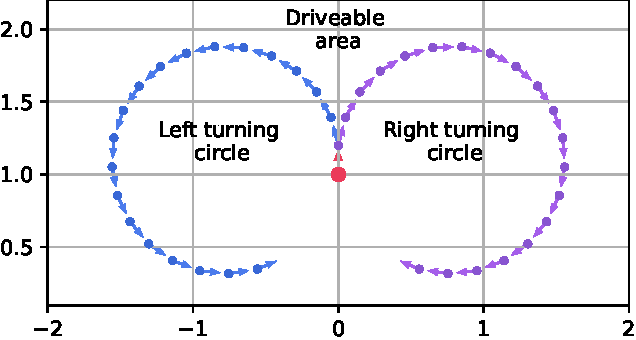
\includegraphics[width=0.9\linewidth]{Imgs/tuning_angle.pdf}
    \caption{The left and right tuning circles for a vehicle pointing upwards.}
    \label{fig:tuning_angle}
\end{figure}

The driveable area of the vehicle, lies in the v-shape that separates the two turning circles.
Therefore, for the vehicle to be safe, the track must intersect with the driveable area.

In the derivation, we assume that valid solutions keep the vehicle pointing forwards, towards the right.
Therefore, the vehicle turning backwards is synonymous with the vehicle crashing

\begin{figure}[h]
    \centering
    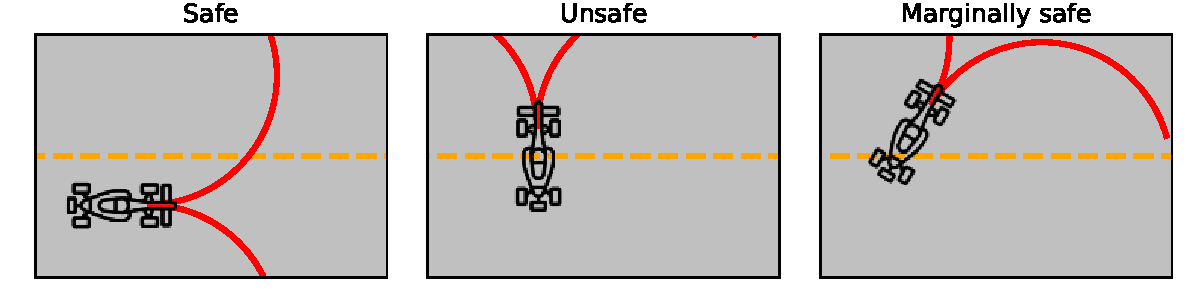
\includegraphics[width=\linewidth]{Imgs/straight_line_safety.pdf}
    \caption{Straight track safe, unsafe and marginally safe scenarios.}
    \label{fig:straight_line_safety}
\end{figure}

Figure \ref{fig:straight_line_safety} shows safe, unsafe and marginally safe scenarios on a straight track.
The first scenario is safe, since the driveable area in front of the vehicle intersects with the track.
The second scenario is unsafe because all of the driveable area leads off the track. 
Therefore, this is an inevitable collision state since the vehicle will definitely crash, irrespective of the actions selected.
The third state is marginally safe, meaning that it is on the boundary of safety.
The theory of barriers says that the barrier is defined by the path being range.
Therefore, the limit of safety is when the tuning circle is tangent to the track limit.
In the third image, the turning circle is tangent to the track boundary.

\textbf{Defining Marginal Safety:}
To determine if a state is safe or unsafe, we must calculate if it lies inside or outside the marginally safe zone.
This is done by using the geometric properties of the circle to calculate if there is enough space on the track for the vehicle to turn.
Since the track is straight and considered to be infinitely long, the only two decision variables are the verticle position $y$ and the orientation angle $\theta$.
For a given $y$ and $\theta$ pair, the problem is to determine if the vehicle is safe or unsafe.

Since the track is straight, the tangent to the track is always in the horizontal direction.
Therefore, the safety can be checked by drawing the turning circle and considering if there is enough verticle space for the turning circle direction to become horizontal.
Figure \ref{fig:tangent_circles} visually shows this by example.


\begin{figure}[h]
    \centering
    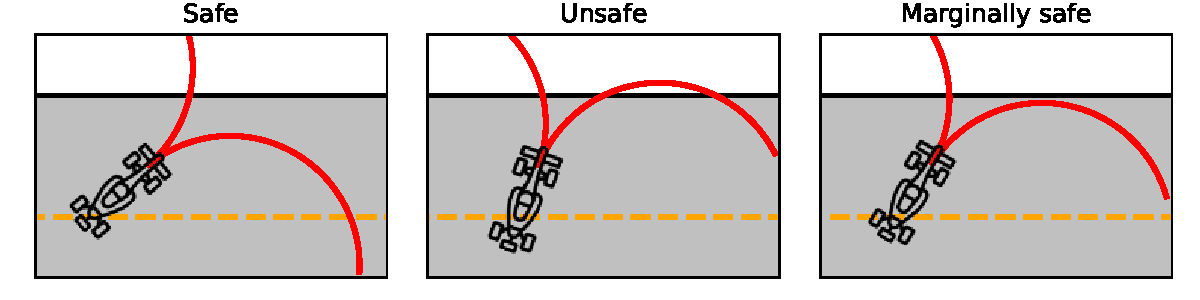
\includegraphics[width=\linewidth]{Imgs/tangent_circles.pdf}
    \caption{Straight track safe, unsafe and marginally safe scenarios.}
    \label{fig:tangent_circles}
\end{figure}

In Figure \ref{fig:tangent_circles}, the first scenario is safe because the right turning circle fits into the track.
The second scenario does not have enough verticle space for the vehicle to turn; thus, the circle exceeds the track.
Finally, the marginal safety has the turning circle tangent to the track.

\begin{figure}
    \centering
    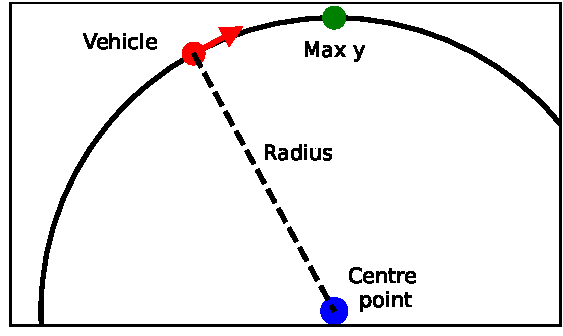
\includegraphics[width=0.8\linewidth]{Imgs/CircleGeometry.pdf}
    \caption{Geometry of the vehicle defined by the turning circle.}
    \label{fig:CircleGeometry}
\end{figure}

Figure \ref{fig:CircleGeometry} shows how the turning circle of car can be analytically defined.
The radius $R$ is given by, 
\begin{equation}
    R = \frac{L}{\tan(\delta)}
\end{equation}
where $L$ is the vehicle wheelbase and $\delta$ is the steering angle.
Since the maximum steering angle for a vehicle is a constant, the radius is also a constant. 
The circle's centre point is calculated using the vehicle orientation as a tangent to the circle, and the radius.
The centre points are calculated as,
\begin{align}
    x_c & = x + R \cos(\pi/2 - \theta) \\
    y_c & = y + R \sin(\pi/2 - \theta) 
\end{align}
The highest point of the circle is then calculated as $y_c + R$.
If this point is smaller than the maximum track height, the vehicle is safe.
Otherwise, the vehicle is unsafe.

\textbf{Straight Line Safety Psuedo Code:}
The safety algorithm is shown in Algorithm \ref{fig:straight_line_safety}.

\begin{algorithm}
    \caption{Straight line safety algorithm} \label{alg:straight_safety}
    \begin{algorithmic}[1]
        \State Calculate the next state 
        \State Calculate the circle centre point
        \State Calculate track height required 
        \If{$h_\text{required} > h_\text{track}$}
            \State result = unsafe
        \Else 
            \State result = safe
        \EndIf
    \end{algorithmic}
\end{algorithm}



\subsection{Curved Tracks}


\subsection{Vehicle Speed}

\section{Evaluation}




\section{Conclusion}

Ending 

\addtolength{\textheight}{-12cm}   % This command serves to balance the column lengths
                                  % on the last page of the document manually. It shortens
                                  % the textheight of the last page by a suitable amount.
                                  % This command does not take effect until the next page
                                  % so it should come on the page before the last. Make
                                  % sure that you do not shorten the textheight too much.


\typeout{}

\bibliographystyle{IEEEtran}
\bibliography{IEEEabrv,ref}




\end{document}
